%%%%%%%% ICML 2019 EXAMPLE LATEX SUBMISSION FILE %%%%%%%%%%%%%%%%%

\documentclass{article}

% Recommended, but optional, packages for figures and better typesetting:
\usepackage{microtype}
\usepackage{graphicx}
\usepackage{subfigure}
\usepackage{booktabs} % for professional tables
\usepackage{natbib}
\usepackage{graphicx}
\usepackage{amsmath}
\usepackage{amssymb}
\usepackage{multirow}
\usepackage{mathabx}
\usepackage{optidef}

%\usepackage{subcaption}

% hyperref makes hyperlinks in the resulting PDF.
% If your build breaks (sometimes temporarily if a hyperlink spans a page)
% please comment out the following usepackage line and replace
% \usepackage{icml2019} with \usepackage[nohyperref]{icml2019} above.
\usepackage{hyperref}

% Attempt to make hyperref and algorithmic work together better:
\newcommand{\theHalgorithm}{\arabic{algorithm}}

\usepackage{array,tabularx}
\newenvironment{vardefs*}{\par\vspace{\abovedisplayskip}\noindent
   \tabularx{\columnwidth}{>{$}l<{$} @{${}:{}$} >{\raggedright\arraybackslash}X}}
  {\endtabularx\par\vspace{\belowdisplayskip}}
  
 \everymath{\displaystyle} 

% Use the following line for the initial blind version submitted for review:
\usepackage{icml2019}

% If accepted, instead use the following line for the camera-ready submission:
%\usepackage[accepted]{icml2019}

% The \icmltitle you define below is probably too long as a header.
% Therefore, a short form for the running title is supplied here:
\icmltitlerunning{Vehicle Routing Problem}
\begin{document}

\twocolumn[
\icmltitle{Vehicle Routing Problem}

% It is OKAY to include author information, even for blind
% submissions: the style file will automatically remove it for you
% unless you've provided the [accepted] option to the icml2019
% package.

% List of affiliations: The first argument should be a (short)
% identifier you will use later to specify author affiliations
% Academic affiliations should list Department, University, City, Region, Country
% Industry affiliations should list Company, City, Region, Country

% You can specify symbols, otherwise they are numbered in order.
% Ideally, you should not use this facility. Affiliations will be numbered
% in order of appearance and this is the preferred way.
\icmlsetsymbol{equal}{*}

\begin{icmlauthorlist}
\icmlauthor{John Doe}{equal,to}
\end{icmlauthorlist}

\icmlaffiliation{to}{AWS Sagemaker RL}
\icmlcorrespondingauthor{John Doe}{}
%\icmlcorrespondingauthor{Eee Pppp}{ep@eden.co.uk}

% You may provide any keywords that you
% find helpful for describing your paper; these are used to populate
% the "keywords" metadata in the PDF but will not be shown in the document
\icmlkeywords{Machine Learning, ICML}

\vskip 0.3in
]

% this must go after the closing bracket ] following \twocolumn[ ...

% This command actually creates the footnote in the first column
% listing the affiliations and the copyright notice.
% The command takes one argument, which is text to display at the start of the footnote.
% The \icmlEqualContribution command is standard text for equal contribution.
% Remove it (just {}) if you do not need this facility.

%\printAffiliationsAndNotice{}  % leave blank if no need to mention equal contribution
\printAffiliationsAndNotice{\icmlEqualContribution} % otherwise use the standard text.

\begin{abstract}
\end{abstract}

\section{Vehicle Routing Problem}
\label{sec_vrp_intro}

The traveling salesman problem (TSP), which involves finding the shortest route that visits each node in a graph exactly once and returns to the starting node, is one of the most widely studied problems in combinatorial optimization both due to its NP-hard nature and as well as its practical applications (**waterloo page). Vehicle routing problem (VRP) is a generalization of TSP where one or more vehicles are expected to visit the nodes in a graph, usually to satisfy customer demand. VRP is also a well studied topic and has very important applications, especially in supply chain and logistics. These real-life applications lead to many variants of VRP with different constraints, such as  capacitated vehicles, pickups and deliveries on the route, time windows associated with each pickup and delivery etc. 

An important extension of VRP is one with some of the information about the graph is revealed over time, such as demand and travel time. This class of VRP is called dynamic VRP (DVRP, also known as real-time or online VRP). A stochastic VRP (SVRP) is where one or more  problem parameters are stochastic with some known probability distributions. In a lot of real-life applications, the VRP on hand is both stochastic and dynamic (SDVRP), which is also focus of this work. We formulate a variant of SVRP and compare solution approaches from the Operations Research (OR) and Reinforcement Learning (RL) literature.

\subsection{Problem Formulation}
\label{sec_vrp_pf}
We consider a version of the VRP that is of a food delivery driver (e.g. an Amazon Restaurants driver). Orders arrive at the driver's phone app over time in a dynamic manner. Each order has a reward (e.g. delivery fee and tip) associated with it, known to the driver at the time of order creation, and it is assigned to one of the restaurants in the city. "City" here means the whole Euclidean space in which the VRP problem lives. The city consists of mutually exclusive regions that generate orders at different rates and with rewards according to probability distributions with different parameters. Each order needs to be delivered within a certain time limit, which starts with the order creation and same for all orders. The driver has to accept an order and pick it up from the associated restaurant prior to delivery. Any order that has not been accepted yet by the driver disappears probabilistically earlier than the time limit, implying a competitive environment in which other drivers could accept the open orders. There is a capacity on the number of orders the driver can carry in the vehicle, however there is no limit on the number of orders that are accepted (but not picked up or delivered) by the driver at the same time. Finally, there is a cost associated with each time step that passes and an additional variable cost for the distance traveled. The driver's goal is to maximize the total net reward over an episode.

This problem is known as stochastic and dynamic capacitated vehicle routing problem with pickup and delivery, time windows and service guarantee. (SDPDPTW with service guarantee).

\subsection{Related Work}
Over the past few years, reinforcement learning methods have been successfully used for solving combinatorial optimization problems, including Traveling Salesman Probelm (TSP), Vehicle Routing Problem (VRP), and knapsack. Bello et al. \cite{bello2016neural} employ a pointer network \cite{vinyals2015pointer} to optimize the policy, and the neural architecture comprises an LSTM encoder-decoder coupled with an attention mechanism. Using negative tour length as the reward signal, they train the LSTM network by an Acgtor-Critic algorithm. Although the framework works good for TSP and knapsack, it assumes the system representation is static, which is not the case in VRP. 

%Instead of using separate encoder and decoder, Dai et al. \cite{khalil2017learning} develop a single model based on graph embeddings. They use DQN algorithm to train the greedy policy and the graph embedding network simulateously. The performance is comparable to the pointer network \cite{bello2016neural} for the TSP task. However, since VRP allows the depot to be visited multiple times, their proposed framework does not directly apply here.

In the context of VRP task, Kool et al. \cite{kool2018attention} develops a model fully based on attention layers, which utilizes the Transformer architecture \cite{vaswani2017attention} as the ecoder and includes an extra attention layer as the decoder. Their proposed model is trained by policy gradients with a greedy baseline, and evaluated on both standard Capacitated VRP (CVRP) and Split Deliverry VRP (SDVRP).  Nazari et al. \cite{nazari2018reinforcement} directly use the embedded inputs instad of a recurrent network for the input. After using the Actor-Critic alogorithm for training, the ouput node can be chosen both greedily or by beam search. In addition to CVRP and SDVRP, the authors also allow the customers and their demands to be stochastic.

Compared to the aforementioned work, there are three important differences in our reinforcement learning solution. First, the reward is formulated from a distinct point of view. While traditional VRP focus on minimizing the tour length, we extend this criteria to integrate order values to learn if the agent is able to prioritize profitable orders. Second, we are interested in considering a more complex and realistic environment, for example, multiple zones with various order generation frequency. This can yield a substantial change of route over time, and we wish to evaluate whether RL can accommodate accordingly. Third, our model uses a simple fully connected network instead of the pointer network or attention mechanism. We do not aim to outperm the algorithms with specilized neural architectures. Rather, we want to benchmark the performance of RL solution with a basic structure. We encourage furthur dive into this problem.

\subsection{Baseline Algorithm}
In order to get a baseline solution, we use the classical three-index Mixed Integer Programming formulation (see \cite{LuDessouky2004}, \cite{RopkeCordeau2009} and \cite{FURTADO2017334}).

\subsubsection*{Sets}
\begin{vardefs*}
V & Current vehicle location, $V=\{0\}$ \\
P & Pickup nodes (copies of the restaurant nodes, associated with the orders that are not in transit)  \\
D & Delivery nodes representing the orders that are not in transit, $D = \{j | j= i + n, i \in P, n=|P| \}$  \\
A & Nodes representing the orders that are accepted by the driver; $A \subset D$ \\
T & Delivery nodes representing the orders that are in transit  \\
R & Nodes representing the restaurants, used for final return) \\
N & Set of all nodes in the graph, $N = V \cup P \cup D  \cup T \cup R $\\
E & Set of all edges, $E=\{(i, j),  \forall i, j \in N\}$
\end{vardefs*}


\subsubsection*{Decision variables}
\begin{vardefs*}
 x_{ij} & Binary variable, 1 if the vehicle uses the arc from node $i$ to $j$, 0 otherwise; $i, j \in N$ \\
y_{i}  & Binary variable, 1 if the order $i$ is accepted, 0 otherwise; $i \in P$\\
Q_{i} & Auxiliary variable to track the capacity usage as of node  $i$; $i \in N$ \\ 
B_{i} & Auxiliary variable to track the time as of node  $i$; $i \in N$
\end{vardefs*}

\subsubsection*{Parameters}
\begin{vardefs*}
n & Number of orders available to pick up, $n = |P|$ \\ 
c_{ij} & Symmetric Manhattan distance (in miles) matrix between node $i$ and $j$, $(i, j) \in E$ \\
q_i & Supply (demand) at node $i$, $q_0 = |T|; q_i = 1, \forall i \in P;  q_i = -1, \forall i \in D \cup T; q_i = 0 \in R$  \\ 
l_i & Remaining time to deliver order $i$, $i \in D \cup T$ \\ 
m & Travel cost per mile \\
r_i & Revenue for order associated with pick up node $i$, $i \in P$  \\
U & Vehicle capacity  \\
M & A very big number  \\ 
t & Time to travel one mile  \\
d & A constant positive service time spent on accept, pickup, delivery
\end{vardefs*}

\subsubsection*{Model}
\begin{equation}
\begin{array}{rrclcl}
& \max_{x, y, Q, B} & \multicolumn{3}{l}{ \sum_{i \in P} r_i y_i - m \sum_{(i,j) \in E} c_{ij} x_{ij}  } \\  
& \textrm{s.t.} \qquad  \sum_{j \in N} x_{ij}   &=& y_i & \forall i \in P \\   %leave
& \sum_{j \in N} x_{ij} - \sum_{j \in N} x_{i+n,j}  & = & 0 & \forall i \in P  \\     %pickup
& y_i & =& 1 & \forall i \in A \\  % accepted
& \sum_{j \in N} x_{ij}   &=& 1 & \forall i \in V \cup T \\  % start and  in-transit
& \sum_{i \in N \setminus R } \sum_{j \in R }  x_{ij}   &=& 1  &\\     %end 
& \sum_{j \in N \setminus R } x_{ji} - \sum_{j \in N} x_{ij}  & = & 0 & \forall i \in P \cup D \cup T  \\     %flow
& Q_i + q_j - M (1-x_{ij} ) &\leq& Q_j & \forall i,j \in N \\  %captrack
& \max{(0, q_i)}    &\leq& Q_i & \forall i \in N \\  %cap_lb
& \min{(U, U+q_i)}    &\geq& Q_i & \forall i \in N \\  %cap_ub
& B_i + d + c_{ij} t -  M (1-x_{ij} )  &\leq& B_j   & \forall i,j \in N \\  %time_track , *\mathcal{1}\{ i \notin V  \}
& B_i +  c_{i, i+n} t -  M (1- y_i )  &\leq& B_{i+n}  & \forall i \in P \\ %precedence
&  d \sum_{i \in P \setminus A}  y_i  & = & B_0  \\ %timetoaccept
& B_i  &\leq& l_i  & \forall i \in D \cup T \\ %precedence
& x_{ij}, y_i &\in& \{0, 1\} & \forall i,j \in N  \\ 
\end{array}
\end{equation}


\subsection{Reinforcement Learning Algorithm}
We consider the Markov Decision Process (MDP) formulation to tackle this problem and cast the optimal routing path as a sequence of actions that an agent takes. To map the scenario described in \ref{sec_vrp_pf} succinctly, we include three components in the state -- restaurant location, driver info, and order info. The driver info contains the driver's position, the maximum number of orders can be carried at one time, and the capacity left. For each request, the agent is aware of the order's location and status. The order info also contains the time elapsed since each order's generation and the corresponding dollar value. 

At every timestep, the agent can choose an action from five options -- accept an order, pick up an accepted order, go to a customer's node for delivery, head to a specific restaurant, or wait and stay unmoved. Note that the vehicle's capacity remains unchanged if an order is accepted but not picked up. In effect, this grants agent the flexibility to accept more orders than its capicity, and thus it can pick up later when space allows. The action of heading to a specifc restaurant is motivated by the desire for learning hot nodes. From a practical perspective, in case where majority of the customer orders comes from a highly rated cafe, we wish to teach the agent to stay around this cafe even when there are currently no orders.

Given the set of restaurants and stochastic orders, we are interested in earning a maximum income, which maps to the reward in RL study. The reward is set as the total value of all delivered orders minus the penalty, and the value is divided into $3$ equal parts to encourage order acceptance as well as delievery. More specifically, each part is assigned to the agent when the order gets accepted, picked up, and delievered respectively.  As for the penalty, we consider a cost both per move and per timestep to mimic the real world. A large penalty is imposed additionally if the agent accepts an order but fails to deliver within the promise time. This way, we expect the learned policy to be capable of not only making full usage of its capacity, but also avoiding unsuccessful deliveries. 

In order to generate feasible actions, we have used a soft masking scheme which forces an action conversion under invalid scenarios. The masking is soft in the sense that there's no constraint on the policy training, and we check the generated actions at each step in an ad-hoc manner. Particularly, the move is converted to `wait' regardless of the policy output if the agent tries to perform the following actions: \textit{(i)} pick up an order when its remaining capacity is $0$; \textit{(ii)} pick up an order that is not yet accepted; \textit{(iii)} deliver an order that is not yet picked up. 

To train the policy, we apply the APE-X \cite{horgan2018distributed} DQN \cite{mnih2013playing} algorithm due to its scaling capability by generating more experience replays and picking from them in a distributed prioritized fashion. In principle, there are multiple actors that predict the next action probability distribution, each with its own policy and instance of the environment. Then the single critic samples from the shared experience replay memory and updates the network with multi-step bootstrap return. We feed the input into a fully connected layer with 256 hidden units to compute the Q values for each action, and the networks are updated periodically with the latest parameters from the critic.  






\subsection{Gym Environment}

By



\subsection{Results}
\begin{figure}[h!]
	\centering
	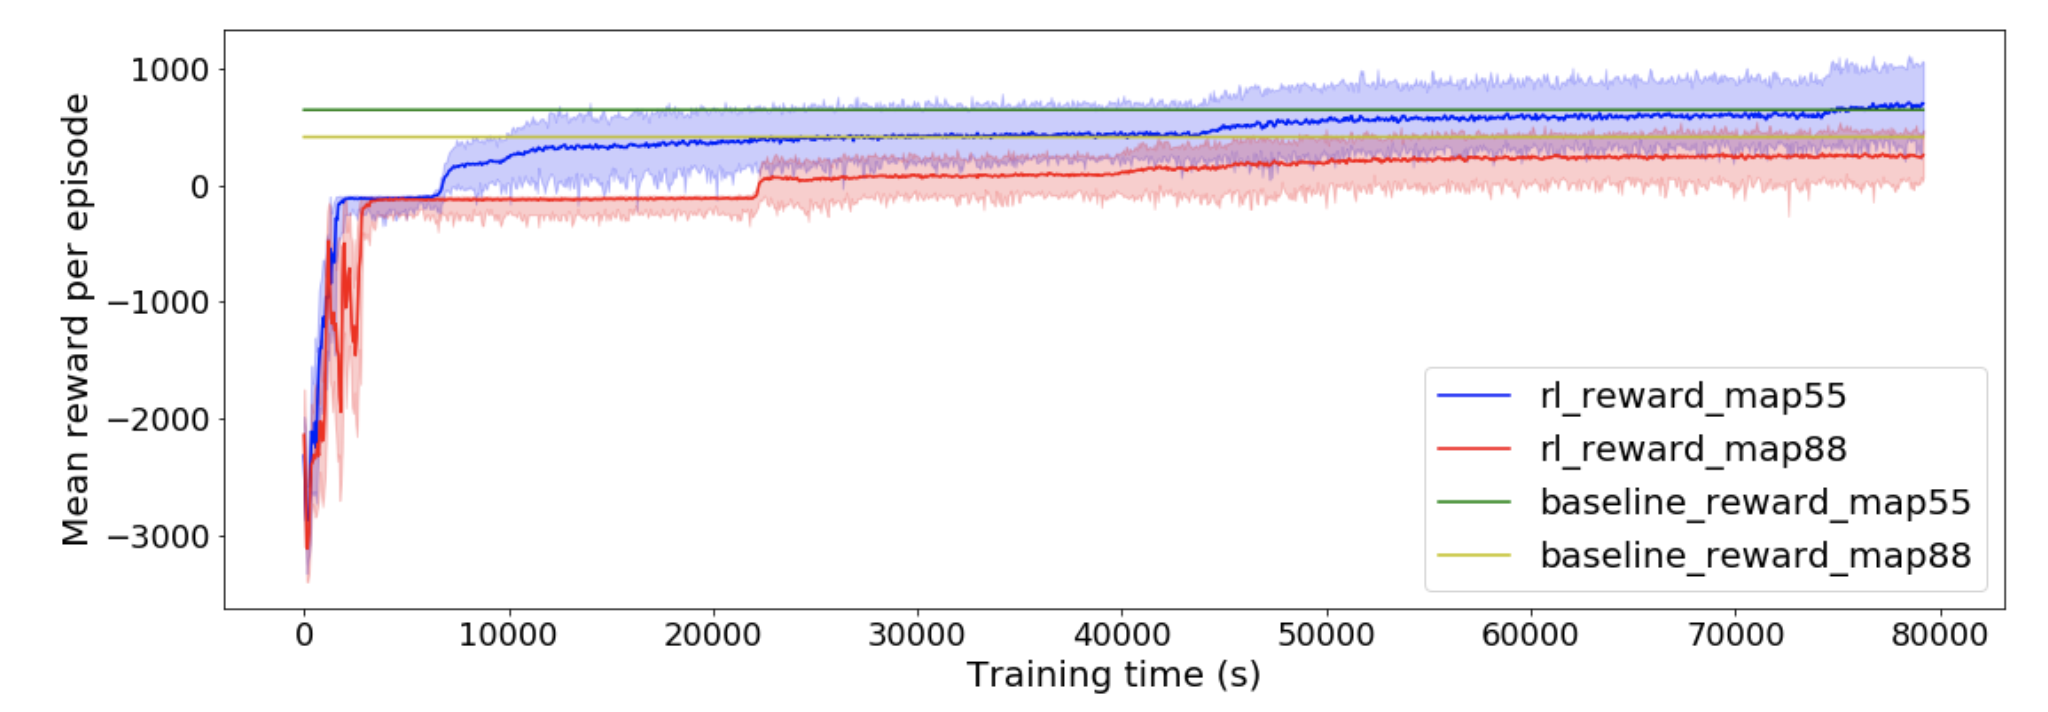
\includegraphics[width=1\linewidth]{vrp_images/different_map_size.png}
	\caption{RL vs baseline solution for ...}
	\label{fig:vrp_map_size}
\end{figure}

\begin{figure}[h!]
	\centering
	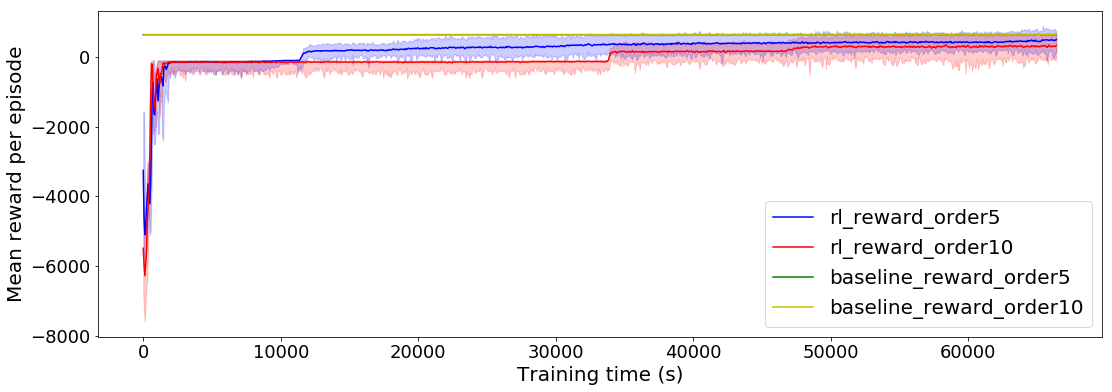
\includegraphics[width=1\linewidth]{vrp_images/different_order_number.png}
	\caption{RL vs baseline solution for ...}
	\label{fig:vrp_order_number}
\end{figure}

\begin{figure}[h!]
	\centering
	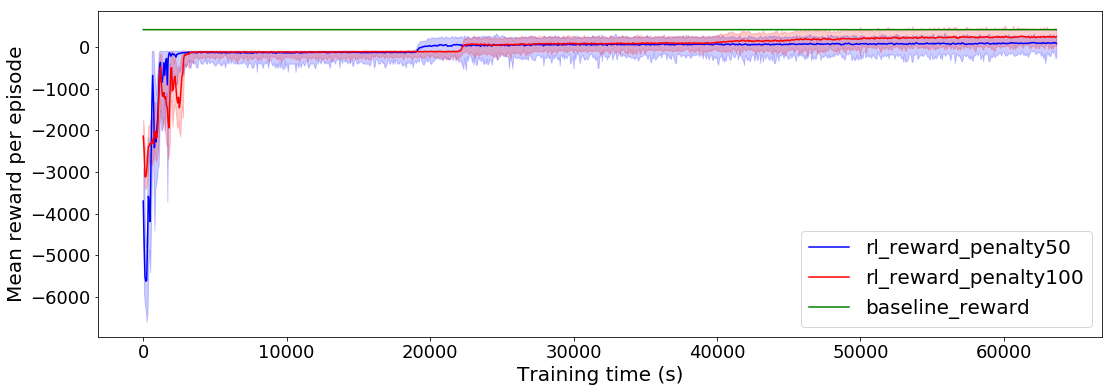
\includegraphics[width=1\linewidth]{vrp_images/different_penalty.png}
	\caption{RL vs baseline solution for ...}
	\label{fig:vrp_penalty}
\end{figure}


% In the unusual situation where you want a paper to appear in the
% references without citing it in the main text, use \nocite
%\nocite{langley00}

\bibliography{refs_vrp}
\bibliographystyle{icml2019}


%%%%%%%%%%%%%%%%%%%%%%%%%%%%%%%%%%%%%%%%%%%%%%%%%%%%%%%%%%%%%%%%%%%%%%%%%%%%%%%
%%%%%%%%%%%%%%%%%%%%%%%%%%%%%%%%%%%%%%%%%%%%%%%%%%%%%%%%%%%%%%%%%%%%%%%%%%%%%%%
% DELETE THIS PART. DO NOT PLACE CONTENT AFTER THE REFERENCES!
%%%%%%%%%%%%%%%%%%%%%%%%%%%%%%%%%%%%%%%%%%%%%%%%%%%%%%%%%%%%%%%%%%%%%%%%%%%%%%%
%%%%%%%%%%%%%%%%%%%%%%%%%%%%%%%%%%%%%%%%%%%%%%%%%%%%%%%%%%%%%%%%%%%%%%%%%%%%%%%
\appendix
\section{Do \emph{not} have an appendix here}

\textbf{\emph{Do not put content after the references.}}
%
Put anything that you might normally include after the references in a separate
supplementary file.

We recommend that you build supplementary material in a separate document.
If you must create one PDF and cut it up, please be careful to use a tool that
doesn't alter the margins, and that doesn't aggressively rewrite the PDF file.
pdftk usually works fine. 

\textbf{Please do not use Apple's preview to cut off supplementary material.} In
previous years it has altered margins, and created headaches at the camera-ready
stage. 
%%%%%%%%%%%%%%%%%%%%%%%%%%%%%%%%%%%%%%%%%%%%%%%%%%%%%%%%%%%%%%%%%%%%%%%%%%%%%%%
%%%%%%%%%%%%%%%%%%%%%%%%%%%%%%%%%%%%%%%%%%%%%%%%%%%%%%%%%%%%%%%%%%%%%%%%%%%%%%%


\end{document}


% This document was modified from the file originally made available by
% Pat Langley and Andrea Danyluk for ICML-2K. This version was created
% by Iain Murray in 2018, and modified by Alexandre Bouchard in
% 2019. Previous contributors include Dan Roy, Lise Getoor and Tobias
% Scheffer, which was slightly modified from the 2010 version by
% Thorsten Joachims & Johannes Fuernkranz, slightly modified from the
% 2009 version by Kiri Wagstaff and Sam Roweis's 2008 version, which is
% slightly modified from Prasad Tadepalli's 2007 version which is a
% lightly changed version of the previous year's version by Andrew
% Moore, which was in turn edited from those of Kristian Kersting and
% Codrina Lauth. Alex Smola contributed to the algorithmic style files.
